% TNSRE Manuscript — Negative Result
% Self-Supervised Pretraining Does Not Rescue Zero-Shot Cross-Sensor
% Rehabilitation Quality Assessment
%
% IEEEtran conference/journal template
% Use: pdflatex manuscript.tex

\documentclass[10pt,journal]{IEEEtran}

\usepackage{cite}
\usepackage{amsmath,amssymb,amsfonts}
\usepackage{graphicx}
\usepackage{textcomp}
\usepackage{booktabs}
\usepackage{multirow}
\usepackage{array}
\usepackage{hyperref}

\hyphenation{self-su-per-vised pre-training trans-fer re-ha-bi-li-ta-tion}

\begin{document}

\title{Self-Supervised Pretraining Does Not Rescue\\%
Zero-Shot Cross-Sensor Rehabilitation\\%
Quality Assessment}

\author{Sayed~Ashraful~Islam~Opin~\IEEEmembership{Student Member, IEEE}
        and~Shafin~Rahman~\IEEEmembership{Member, IEEE}%
\thanks{This work was supported by ...}
\thanks{S.~A.~I.~Opin and S.~Rahman are with the Department of Electrical and Computer Engineering, North South University, Dhaka, Bangladesh (e-mail: ...).}}

\maketitle

% ===================================================================
\begin{abstract}
Automated rehabilitation quality scoring from skeleton sequences promises objective, scalable assessment, but prior work evaluates exclusively within-dataset under standard cross-validation. We ask whether self-supervised pretraining on unlabeled skeletons from a different sensor enables zero-shot cross-sensor scoring. We pretrain contrastive and masked-motion encoders on 1,000 unlabeled IntelliRehabDS (Kinect v2) sequences, then evaluate on KIMORE (Kinect v2, $N=380$, 77 subjects, leave-one-subject-out) and zero-shot on two independent labeled corpora with different sensors: REHAB246 (OptiTrack, 1,057 reps) and UI-PRMD (Kinect, 2,000 reps). The result is a clean negative across four axes:
(1) zero-shot AUROC is at chance (0.51--0.53) on both corpora; a naive path-length-plus-speed baseline nominally leads (AUROC = 0.55 and 0.54), but under a bootstrap over the ten target subjects the learned models are statistically indistinguishable from chance and the naive baseline's advantage over them is largely not significant;
(2) under a fully-powered 77-fold leave-one-subject-out evaluation, SSL fine-tuning is statistically indistinguishable from training from scratch ($p > 0.3$, Holm-corrected), while SSL linear-probing is significantly \emph{worse} (adjusted $p < 10^{-13}$);
(3) quadrupling the unlabeled pool to approximately 5,000 sequences does not close the gap; and
(4) contrastive and masked-motion paradigms are statistically equivalent ($p = 0.80$).
Degeneracy gates ($\text{pred\_SD} > 0.10$) and probe-sanity checks rule out collapsed models or undertrained encoders as explanations. A sensor-identity probe recovers the acquisition sensor with \emph{perfect} accuracy from both TCN and ST-GCN features (1.00 vs.\ 0.33 chance), localizing the failure to sensor-entangled representations; and the null persists under a spatial-prior ST-GCN backbone, a bone-length-preserving joint-vector input, and domain adaptation and generalization (AdaBN, DANN, SWAD).
The barrier is compound domain shift --- differing sensors, acquisition protocols, and exercise-type compositions --- that SSL pretraining cannot bridge on its own: the null is stable across pretext tasks, pool sizes, evaluation protocols, and two independent test corpora.
We conclude that SSL pretraining on unlabeled skeletons does not confer cross-sensor transferability for rehabilitation scoring, and recommend that the field prioritize sensor-invariant representations over more sophisticated SSL on a single sensor modality.
\end{abstract}

\begin{IEEEkeywords}
Self-supervised learning, rehabilitation quality assessment, zero-shot transfer, KIMORE, domain shift, leave-one-subject-out.
\end{IEEEkeywords}

% ===================================================================
\section{Introduction}
\label{sec:intro}

Automated quality assessment of rehabilitation exercises from skeleton sequences has the potential to enable objective, remote, and continuous monitoring of physical therapy outcomes, replacing or augmenting subjective in-clinic physiotherapist scoring \cite{capecci2019kimore}. The KIMORE dataset \cite{capecci2019kimore} has emerged as the primary benchmark for this task: 78 subjects performing five trunk and hip exercises, each scored 0--50 by a physician. Published Spearman rank correlations on KIMORE range from 0.70 to as high as 0.965 \cite{karlov2024,abedi2023,kuang2026}.

All existing work, however, evaluates under ideal conditions: within-dataset, with the training and test sets drawn from the same sensor, under the same acquisition protocol, and with standard $k$-fold cross-validation that permits subject-identity leakage. This leaves a critical gap: real-world deployment requires generalization across sensor types --- a Kinect v2 in a hospital, a webcam in a patient's home, a marker-based motion capture system in a specialized clinic. No prior study tests whether self-supervised pretraining on unlabeled target-sensor data can bridge this gap without any labeled target-sensor examples.

In this paper we present, to our knowledge, the first systematic evaluation of self-supervised pretraining for zero-shot cross-sensor rehabilitation quality assessment. Our contributions are:

\begin{enumerate}
    \item \textbf{A robust negative result:} SSL pretraining on unlabeled skeletons does not enable zero-shot cross-sensor transfer. Across two pretext tasks (contrastive and masked-motion), two pool sizes ($\sim$1,000 and $\sim$5,000 unlabeled sequences), two independent labeled test corpora (REHAB246, OptiTrack; UI-PRMD, Kinect), and two evaluation protocols (5-fold and 77-fold leave-one-subject-out), every condition scores at chance (AUROC 0.51--0.53). A simple naive kinematic baseline (AUROC 0.55/0.54) nominally leads, but a bootstrap over the ten target subjects shows the learned models are statistically indistinguishable from chance and the naive baseline's advantage over them is largely not significant (Table~\ref{tab:auroc-sig})---no method, learned or naive, achieves subject-level-meaningful cross-sensor discrimination.
    \item \textbf{Within-domain evidence of the same null:} under a fully-powered 77-fold leave-one-subject-out (LOSO) evaluation with sample-level statistics ($N=380$), SSL fine-tuning is statistically indistinguishable from training from scratch, and SSL linear-probing is significantly worse. The two SSL paradigms are statistically equivalent.
    \item \textbf{Rigor safeguards:} we incorporate (a) a degeneracy gate ($\text{pred\_SD} > 0.10$) to detect collapsed near-constant predictors, (b) probe-sanity checks confirming the encoders learned meaningful structure, (c) naive-feature baselines as the simplest possible comparator, and (d) Holm-Bonferroni-corrected sample-level pairwise tests.
    \item \textbf{A mechanistic, architecture-independent diagnosis:} a sensor-identity probe classifies the acquisition sensor with perfect accuracy (1.00 vs.\ 0.33 chance) from both TCN and ST-GCN features, showing the encoders represent \emph{sensor identity} rather than movement quality as the dominant signal. The null is robust to a spatial-prior ST-GCN backbone, a translation-invariant bone-length-preserving joint-vector input, and stronger domain adaptation and generalization (AdaBN, DANN, and flat-minima SWAD), none of which reach the naive baseline.
\end{enumerate}

% ===================================================================
\section{Related Work}
\label{sec:related}

\subsection{KIMORE Benchmarks}
The KIMORE dataset \cite{capecci2019kimore} has been evaluated with multiple architectures under 5-fold cross-validation: Karlov et al.\ \cite{karlov2024} reported mean Spearman $\rho = 0.744$ using an ST-GCN with supervised contrastive learning; Abedi et al.\ \cite{abedi2023} reported $\rho = 0.662$ using cross-modal augmentation; and Kuang et al.\ \cite{kuang2026} reported $\rho = 0.965$ using a dual-stream STGCN. Ismail-Fawaz et al.\ \cite{rehabpile2026} aggregated KIMORE, UI-PRMD, and IRDS under cross-subject splits across nine architectures, reporting MAE and RMSE rather than Spearman correlation. Critically, none of these studies evaluate generalization to a different sensor.

\subsection{Self-Supervised Learning for Skeletons}
SSL for skeleton data has primarily targeted action recognition and classification. Contrastive approaches (SimCLR-style \cite{chen2020simclr}) learn permutation-invariant representations by maximizing agreement between augmented views. Masked-motion approaches (MAE-style \cite{he2022mae}) reconstruct occluded joints from visible context. Both paradigms have shown success within single-sensor settings but have not been tested for zero-shot cross-sensor transfer in rehabilitation.

\subsection{Cross-Sensor Transfer}
Karlov et al.\ \cite{karlov2024} used IRDS for supervised contrastive pretraining followed by fine-tuning on KIMORE --- both Kinect v2 datasets, demonstrating within-modality transfer. No prior work evaluates \emph{zero-shot} cross-sensor transfer (no target-sensor labels of any kind), which is the scenario required when deploying a pretrained model to a new sensor without collecting any labeled data from it.

A large domain adaptation/generalization (DA/DG) literature addresses distribution shift more directly than SSL alone. Feature-alignment methods match source and target statistics---CORAL \cite{sun2016deep} (second-order), MMD-based approaches \cite{long2015dan}, and AdaBN \cite{li2018adabn} (recomputing normalization statistics on the target). Adversarial methods such as DANN \cite{ganin2016dann} learn domain-invariant features via a gradient-reversal domain discriminator. Source-free and test-time methods---SHOT \cite{liang2020shot} and TENT \cite{wang2021tent} (test-time entropy minimization)---adapt without source data or target labels. In parallel, rotation- and scale-invariant input representations (joint-angle/bone-vector features and canonical body models such as SMPL \cite{loper2015smpl}) reduce sensor-induced topology and anthropometric variation at the input. Domain-generalization methods instead seek models that generalize to unseen domains without any target access, e.g.,\ invariant-risk minimization \cite{arjovsky2019irm} and flat-minima weight averaging (SWAD) \cite{cha2021swad}. We evaluate representatives spanning these families---AdaBN, DANN, SWAD, and a joint-angle input representation---alongside SSL to test whether stronger alignment or flat-minima generalization overcomes the compound cross-sensor shift.

% ===================================================================
\section{Methods}
\label{sec:methods}

\subsection{Datasets and Preprocessing}
\label{sec:datasets}

Five datasets are used, summarized in Table~\ref{tab:datasets}.

\begin{table}[t]
\centering
\caption{Datasets used in this study.}
\label{tab:datasets}
\begin{tabular}{lrrrl}
\toprule
Dataset & Subjects & Samples & Joints & Sensor \\
\midrule
KIMORE & 77 & 380 & 25 & Kinect v2 \\
IRDS & 10 & 1,000 & 22$\to$25 & Kinect v2 \\
REHAB246 & 10 & 1,057 & 26$\to$25 & OptiTrack \\
UI-PRMD & 10 & 2,000 & 22$\to$25 & Kinect v2 \\
\bottomrule
\end{tabular}
\end{table}

\textbf{KIMORE} \cite{capecci2019kimore} provides physician-assigned continuous scores (0--50) for 78 subjects performing five exercises (k01, trunk forward flexion; k02, trunk lateral flexion; k03, trunk rotation; k04, hip abduction; k05, hip circumduction). One subject is dropped in preprocessing due to missing data, yielding 77 subjects $\times$ 5 exercises $= 380$ assessment instances. Skeletons are Kinect v2, 25 joints, captured at the sensor's native $\sim$30\,fps and resampled to a common length of 100 frames (see below).

\textbf{IntelliRehabDS (IRDS)} \cite{capecci2019kimore} contains 1,000 unlabeled Kinect v2 sequences (10 subjects $\times$ 10 exercises $\times$ 10 repetitions). IRDS has no correctness or quality labels; it serves exclusively as the SSL pretraining corpus. We pad its 22-joint skeletons to 25 joints (zeros for positions 22--24).

\textbf{REHAB246} \cite{rehab246} is an OptiTrack motion-capture dataset with 1,057 repetitions (558 correct, 499 incorrect) across six exercises and ten subjects, labeled per-repetition for binary movement correctness. This is a \emph{pure cross-sensor} test: OptiTrack is marker-based, unlike the Kinect v2 used for pretraining and KIMORE. We map its 26-joint skeleton to the KIMORE 25-joint layout.

\textbf{UI-PRMD} \cite{vakanski2018uiprmd} provides 2,000 Kinect v2 repetitions (1,000 correct, 1,000 incorrect) across ten exercises and ten subjects. We use identical 22$\to$25 joint padding as for IRDS. UI-PRMD is a \emph{same-sensor, different acquisition} test (Kinect v2, but different placement, room, and population).

\textbf{Exercise overlap across corpora:} KIMORE, IRDS, and UI-PRMD share trunk rotation, hip abduction, and hip circumduction as nominally analogous exercises; IRDS additionally separates left/right variants, while UI-PRMD includes lower-limb exercises (deep squat, hurdle step, lunge) not present in KIMORE. REHAB246 overlaps on trunk rotation and hip abduction only. The cross-sensor evaluation therefore also tests cross-exercise generalization, a factor that compounds the sensor-level shift.

All sequences are resampled to 100 frames via linear interpolation (the native acquisition rate is $\sim$30\,fps for the Kinect~v2 corpora (KIMORE, IRDS, UI-PRMD) with variable per-recording durations, and the external OptiTrack corpus (REHAB246) uses a different native rate; resampling to a common length is standard practice in the KIMORE literature \cite{karlov2024,abedi2023} and enables consistent temporal receptive fields across architectures). Pre-normalization sequence lengths varied from 100--300 frames. After resampling, model inputs are standardized per coordinate using a \texttt{StandardScaler} fit on the training subjects of each fold and applied as a fixed affine transform to every sequence; this centers the training distribution while preserving within-sequence scale and speed structure. We separately ablate strict per-sequence z-scoring (per-sequence mean/standard deviation), which \emph{does} discard per-sequence scale cues, and find it does not change the zero-shot conclusion (Table~\ref{tab:robustness-c}); consistent with this, the naive baseline's small advantage disappears under per-sequence z-scoring (Table~\ref{tab:naive-sens}), indicating that the scale/speed cue it exploits is exactly what strict normalization removes.

\textbf{Joint-space alignment:} The three external corpora use different skeleton topologies from KIMORE's 25-joint Kinect~v2 layout. IRDS and UI-PRMD provide 22 Kinect~v2 joints; we pad with three all-zero joints at positions 22--24 (no anatomical correspondence). REHAB246 provides 26 OptiTrack joints; we apply an anatomically-aligned permutation (\texttt{map\_26\_to\_25}, validated against the official joint naming table) that maps 25 of the 26 OptiTrack markers to their KIMORE counterparts, dropping the clavicle and head-end markers that have no Kinect analogue. All mappings are checked for cross-corpus consistency in bone-length ratios after normalization.

\subsection{Self-Supervised Pretraining}
\label{sec:pretraining}

We pretrain a Temporal Convolutional Network (TCN) encoder \cite{bai2018tcn} --- previously shown to be the highest-performing architecture for KIMORE scoring --- under two SSL paradigms:

\textbf{Contrastive (SimCLR-style):} Each sequence generates two augmented views via random joint jitter, scaling, rotation, flipping, and channel dropout. The encoder maps both views to 128-dimensional embeddings, and the NT-Xent loss \cite{chen2020simclr} maximizes agreement between views of the same sequence while minimizing agreement with other sequences in the batch. Temperature $\tau = 0.1$.

\textbf{Masked-motion (MAE-style):} Fifty percent of joint coordinates are randomly masked (replaced with zeros) at each time step. The encoder processes the unmasked coordinates, and a lightweight decoder reconstructs the full sequence in normalized coordinates under MSE loss \cite{he2022mae}. Masking is applied independently per sample, not per corpus.

Both encoders are TCNs with $d_{\text{model}} = 128$, 4 blocks, dilation pattern $[1,2,4,8]$, kernel size 3, and dropout 0.3. Pretraining runs for 300 epochs, batch size 128, Adam optimizer with learning rate $10^{-3}$. Two pool configurations are tested: \texttt{irds\_only} ($\sim$1,000 sequences, pure cross-sensor) and \texttt{all\_corpora} ($\sim$5,000 sequences including REHAB246 and UI-PRMD, a transductive upper bound). All hyperparameters were fixed before evaluating any zero-shot results; model selection did not use target-distribution information.

\subsection{Evaluation Protocol}
\label{sec:eval}

\textbf{77-fold Leave-One-Subject-Out (LOSO):} Each of the 77 KIMORE subjects is held out as the test set exactly once. This is true LOSO without any subject-identity leakage. All 77 folds share a single fixed split.

\textbf{Five conditions:}
\begin{itemize}
    \item \textbf{A. Scratch:} TCN trained from scratch (random init), no SSL.
    \item \textbf{B. Contrastive LP:} Contrastive encoder frozen; only a linear probe is trained.
    \item \textbf{C. Contrastive FT:} Contrastive encoder fine-tuned end-to-end.
    \item \textbf{D. Masked LP:} Masked-motion encoder frozen; only a linear probe is trained.
    \item \textbf{E. Masked FT:} Masked-motion encoder fine-tuned end-to-end.
\end{itemize}

All conditions use the same TCN regression head (2-layer MLP with a hidden dimension of 64). Training is performed for 100 epochs with batch size 16, Adam optimizer (learning rate $10^{-3}$), and early stopping with patience 100. Out-of-fold (OOF) predictions are pooled across all folds for sample-level analysis ($N = 380$).

\subsection{Zero-Shot Cross-Sensor Evaluation}
\label{sec:zeroshot}

Each model obtained from the 77 LOSO folds is directly evaluated on REHAB246 and UI-PRMD without any retraining or adaptation.

The primary evaluation metric is AUROC, computed between predicted scores and binary correctness labels and averaged across folds. We additionally report the mean rank Spearman correlation and the prediction standard deviation ($\text{pred\_SD}$).

Models with $\text{pred\_SD} < 0.10$ are considered degenerate because they produce nearly constant predictions, making their AUROC values uninformative.

\textbf{Naive kinematic baseline:} Two kinematic features are computed directly from each skeleton sequence:
\begin{itemize}
    \item Total joint path length (sum of Euclidean distances across all joints and frames).
    \item Mean joint speed.
\end{itemize}
The direction-agnostic AUROC of these individual features is computed against the binary correctness labels. Importantly, this baseline does not train any model. No classifier, logistic regression, or optimization procedure is performed. Target labels are used only during evaluation, making this a true zero-shot baseline. AUROC is always computed using the same mapped skeleton sequences as those used by the learned models.

\subsection{Statistical Testing}
\label{sec:stats}

For the within-domain KIMORE evaluation, sample-level paired Wilcoxon signed-rank tests are performed on the absolute prediction errors of matched out-of-fold samples ($N = 380$). All $p$-values are corrected using the Holm--Bonferroni procedure across the ten pairwise condition comparisons.

For each condition, the mean Spearman $\rho$ is reported together with a 95\% confidence interval estimated using a 20-seed stratified bootstrap (500 resamples per seed).

% ===================================================================
\section{Results}
\label{sec:results}

\subsection{Zero-Shot: Chance-Level Everywhere}
\label{sec:zeroshot-results}

Table~\ref{tab:zeroshot} presents the primary result of the paper.

\begin{table}[t]
\centering
\caption{Zero-shot cross-sensor AUROC. \emph{IRDS-only} columns: the SSL encoder is pretrained on the $\sim$1k unlabeled IRDS sequences, then evaluated over all 77 KIMORE LOSO fold models (mean with 95\% CI in parentheses; D = degenerate). \emph{All-corpora} columns: the SSL encoder is pretrained on the pooled $\sim$5k unlabeled sequences of IRDS + KIMORE + REHAB246 + UI-PRMD (target corpora enter as unlabeled pretraining data only --- never with labels), then fine-tuned on all labeled KIMORE data as a single model. In both settings only KIMORE supplies supervision. Every CI excludes 0.55 and lies far below the naive baseline. The naive kinematic baseline is direct AUROC of path-length and speed features (no model trained). CORAL fits a domain-aligned logistic regression on scratch TCN features from KIMORE.}
\label{tab:zeroshot}
\small
\setlength{\tabcolsep}{2.5pt}
\begin{tabular}{@{}lcccc@{}}
\toprule
& \multicolumn{2}{c}{IRDS-only} & \multicolumn{2}{c}{All-corpora} \\
\cmidrule(lr){2-3} \cmidrule(lr){4-5}
Condition & REHAB246 & UI-PRMD & REHAB246 & UI-PRMD \\
\midrule
Scratch         & 0.516 (.003)  & 0.524 (.004) D & 0.513 & 0.527 D \\
Contrast.~LP    & 0.516 (.002)  & 0.518 (.003) D & 0.502 & 0.524 \\
Contrast.~FT    & 0.515 (.003)  & 0.514 (.003)   & 0.503 & 0.509 \\
Masked~LP       & 0.527 (.002)  & 0.512 (.002) D & 0.507 & 0.507 \\
Masked~FT       & 0.519 (.003)  & 0.514 (.002) D & 0.523 & 0.524 \\
\midrule
CORAL           & 0.522 (.003)  & 0.513 (.003)   & ---   & --- \\
\midrule
Naive kinem.    & \textbf{0.554} & \textbf{0.538} & ---   & --- \\
\bottomrule
\end{tabular}
\end{table}

All the learned conditions perform at chance (AUROC 0.51--0.53) on both corpora. Naive kinematic baseline nominally outperforms all SSL conditions on both corpora, at the pool-sample level. However, this ranking is invalid under subject-clustered bootstrap (Table~\ref{tab:auroc-sig}). All the rank Spearman correlations between all the conditions are $|\rho| < 0.03$, confirming the lack of ordinal transfer. Per-fold standard deviations are 0.009--0.017 (95\% CI $\approx \pm 0.003$), confirming the stability of the null hypothesis rather than a statistical fluctuation. AUPRC values (0.51--0.54) replicate the AUROC values, ruling out class imbalance artifacts. CORAL domain adaptation baseline --- aligning second-order statistics of scratch TCN features from the labeled KIMORE data before logistic regression --- is also at chance (AUROC 0.522 and 0.513), confirming that even the source-labeled data cannot alleviate the domain shift via simple feature alignment.

\textbf{Subject-level significance (ten-subject bootstrap).} Because each target corpus has ten subjects only, the repetition-level intervals overestimate the effective sample size. So we re-analyzed all the conditions as well as the naive baseline under a bootstrap sampling subjects rather than repetitions (2000 resamples). Orientation of each score is fixed under the full sample once so that the resampling cannot boost AUROC via taking $\max(\text{AUROC},\,1-\text{AUROC})$ per draw (Table~\ref{tab:auroc-sig}). Under this honest assessment against the subject-level variance, there is no learned model whose AUROC is distinguishable from 0.50 on REHAB246 (chance lies within 95\% subject confidence interval for every model) and only trivial effects exceed chance on UI-PRMD (Scratch 0.527, Contrastive-LP 0.526; both are within 0.03 of chance). The naive baseline, however, exceeds chance on both corpora (REHAB246 0.554, CI [0.506, 0.605], $p = 0.035$; UI-PRMD 0.538, $p < 0.001$), yet its superiority over the learned models is not statistically significant for eight out of ten model $\times$ corpus comparisons ($p = 0.24$--$0.71$); the two exceptions are the fine-tuned SSL variants on UI-PRMD (Contrastive-FT $p = 0.010$, Masked-FT $p = 0.038$), which are not above chance either. Hence, the ordering of Table~\ref{tab:zeroshot} does not survive the subject-level uncertainty: at the subject level, neither the learned models nor the naive baseline can achieve a reliable cross-sensor discrimination.

\begin{table*}[t]
\centering
\footnotesize
\setlength{\tabcolsep}{4pt}
\caption{Subject-clustered AUROC significance. Because each target corpus has only ten subjects, we bootstrap over subject clusters ($2{,}000$ resamples) with each score's orientation fixed once on the full sample. ``$>$chance?'' flags whether the $95\%$ subject CI excludes $0.50$. ``naive$-$model'' is the paired AUROC difference (naive minus that model) with its two-sided bootstrap $p$. No learned model is distinguishable from chance on REHAB246, and the naive baseline's advantage over the learned models is largely not significant.}
\label{tab:auroc-sig}
\begin{tabular}{llccccc}
\toprule
Corpus & Condition & AUROC & 95\% CI (subject) & $p$ vs.\ 0.50 & naive$-$model & $p$(naive$>$model) \\
\midrule
\multirow{6}{*}{REHAB246}
 & Scratch        & 0.515 & [0.467, 0.558] & 0.553 & $+0.040$ & 0.238 \\
 & Contrastive LP & 0.515 & [0.450, 0.581] & 0.631 & $+0.037$ & 0.536 \\
 & Contrastive FT & 0.506 & [0.459, 0.556] & 0.840 & $+0.048$ & 0.253 \\
 & Masked LP      & 0.529 & [0.470, 0.592] & 0.336 & $+0.022$ & 0.706 \\
 & Masked FT      & 0.522 & [0.467, 0.573] & 0.444 & $+0.032$ & 0.356 \\
 & Naive baseline & \textbf{0.554} & [0.506, 0.605] & \textbf{0.035} & --- & --- \\
\midrule
\multirow{6}{*}{UI-PRMD}
 & Scratch        & 0.527 & [0.515, 0.537] & $<$0.001 & $+0.012$ & 0.279 \\
 & Contrastive LP & 0.526 & [0.504, 0.551] & 0.018 & $+0.011$ & 0.570 \\
 & Contrastive FT & 0.508 & [0.490, 0.519] & 0.288 & $+0.031$ & \textbf{0.010} \\
 & Masked LP      & 0.516 & [0.496, 0.540] & 0.103 & $+0.021$ & 0.243 \\
 & Masked FT      & 0.513 & [0.498, 0.529] & 0.083 & $+0.025$ & \textbf{0.038} \\
 & Naive baseline & \textbf{0.538} & [0.520, 0.560] & \textbf{$<$0.001} & --- & --- \\
\bottomrule
\end{tabular}
\end{table*}

The all-corpora column in Table~\ref{tab:zeroshot} shows the transductive upper bound: SSL pretrained on a pool that comprises the unlabeled target corpora. The results are identical --- all the conditions are at chance (AUROC 0.502--0.527) --- confirming that even the direct access to unlabeled target distributions during pretraining does not increase the cross-sensor transfer. This is consistent with the within-domain pool-size ablation (Table~\ref{tab:pool}), which failed to close the gap when increasing the size of the unlabeled pool fourfold.

On REHAB246, all the conditions are non-degenerate ($\text{pred\_SD} > 0.10$); the chance-level AUROC is therefore a real transfer failure rather than a collapse of the predictor. On UI-PRMD, four out of five conditions are degenerate ($\text{pred\_SD} < 0.10$), which indicates that the models collapse to near-constant outputs on this corpus. The non-degenerate scratch condition (SD = 0.12) obtains AUROC = 0.524, still at chance.

\textbf{Per-exercise analysis:} On REHAB246 (six exercises), per-exercise AUROCs of SSL range from 0.53 to 0.64, depending on the pretext task, with minor difference between pretexts. The naive kinematic baseline yields much higher per-exercise AUROCs (0.63--0.87), confirming that simple motion features are exercise-discriminative while SSL encoders fail to use them for cross-sensor discrimination. On UI-PRMD (ten exercises), SSL per-exercise AUROCs vary from 0.52 to 0.71; the maximum values appear on ex1 (deep squat, AUROC up to 0.71) and ex4 (shoulder abduction, AUROC up to 0.62), suggesting a marginal transfer on well-isolated single-joint movements. Crucially, the naive baseline achieves the same or better per-exercise AUROCs on all ten exercises of UI-PRMD. Thus, the per-exercise pattern confirms the aggregate result: SSL does not improve on simple kinematic features at any granularity.

\textbf{Canonicalization ablations:} Application of pelvis-centering and bone-length normalization to the input without retraining did not change any result meaningfully. The best canonicalized condition (contrastive LP on REHAB246) reaches AUROC $0.552 \pm 0.026$, marginally exceeding the naive baseline but having higher variance; all other canonicalized conditions are at chance (AUROC 0.506--0.524). Canonical body model representations alone are not sufficient to close the cross-sensor gap.

\textbf{Sensor encoding probe:} To assess the amount of sensor-specific encoding, we trained a 3-way sensor classifier (KIMORE vs REHAB246 vs UI-PRMD) on scratch TCN features. Balanced accuracy is $1.000 \pm 0.000$ (chance 0.33), and the same perfect separation holds for pairwise discrimination (KIMORE vs REHAB246: 1.00; KIMORE vs UI-PRMD: 1.00). Thus, this confirms that TCN features encode the sensor identity rather than motion content, confirming our claim that SSL learns sensor-specific rather than sensor-invariant structure. This separation is not caused by joint zero-padding: zeroing the padded and duplicated joints ($\{7,11,22,23,24\}$) in all the corpora so that no corpus has a distinguishing pattern of zeros leaves the 3-way probe separated at balanced accuracy 1.000 for both the TCN and the ST-GCN backbone. t-SNE projection of penultimate features (Fig.~\ref{fig:embedding-tsne}) illustrates the separation explicitly: three sensors form well-separated clusters, while correct and incorrect repetitions are mixed within every cluster.

\begin{figure*}[t]
\centering
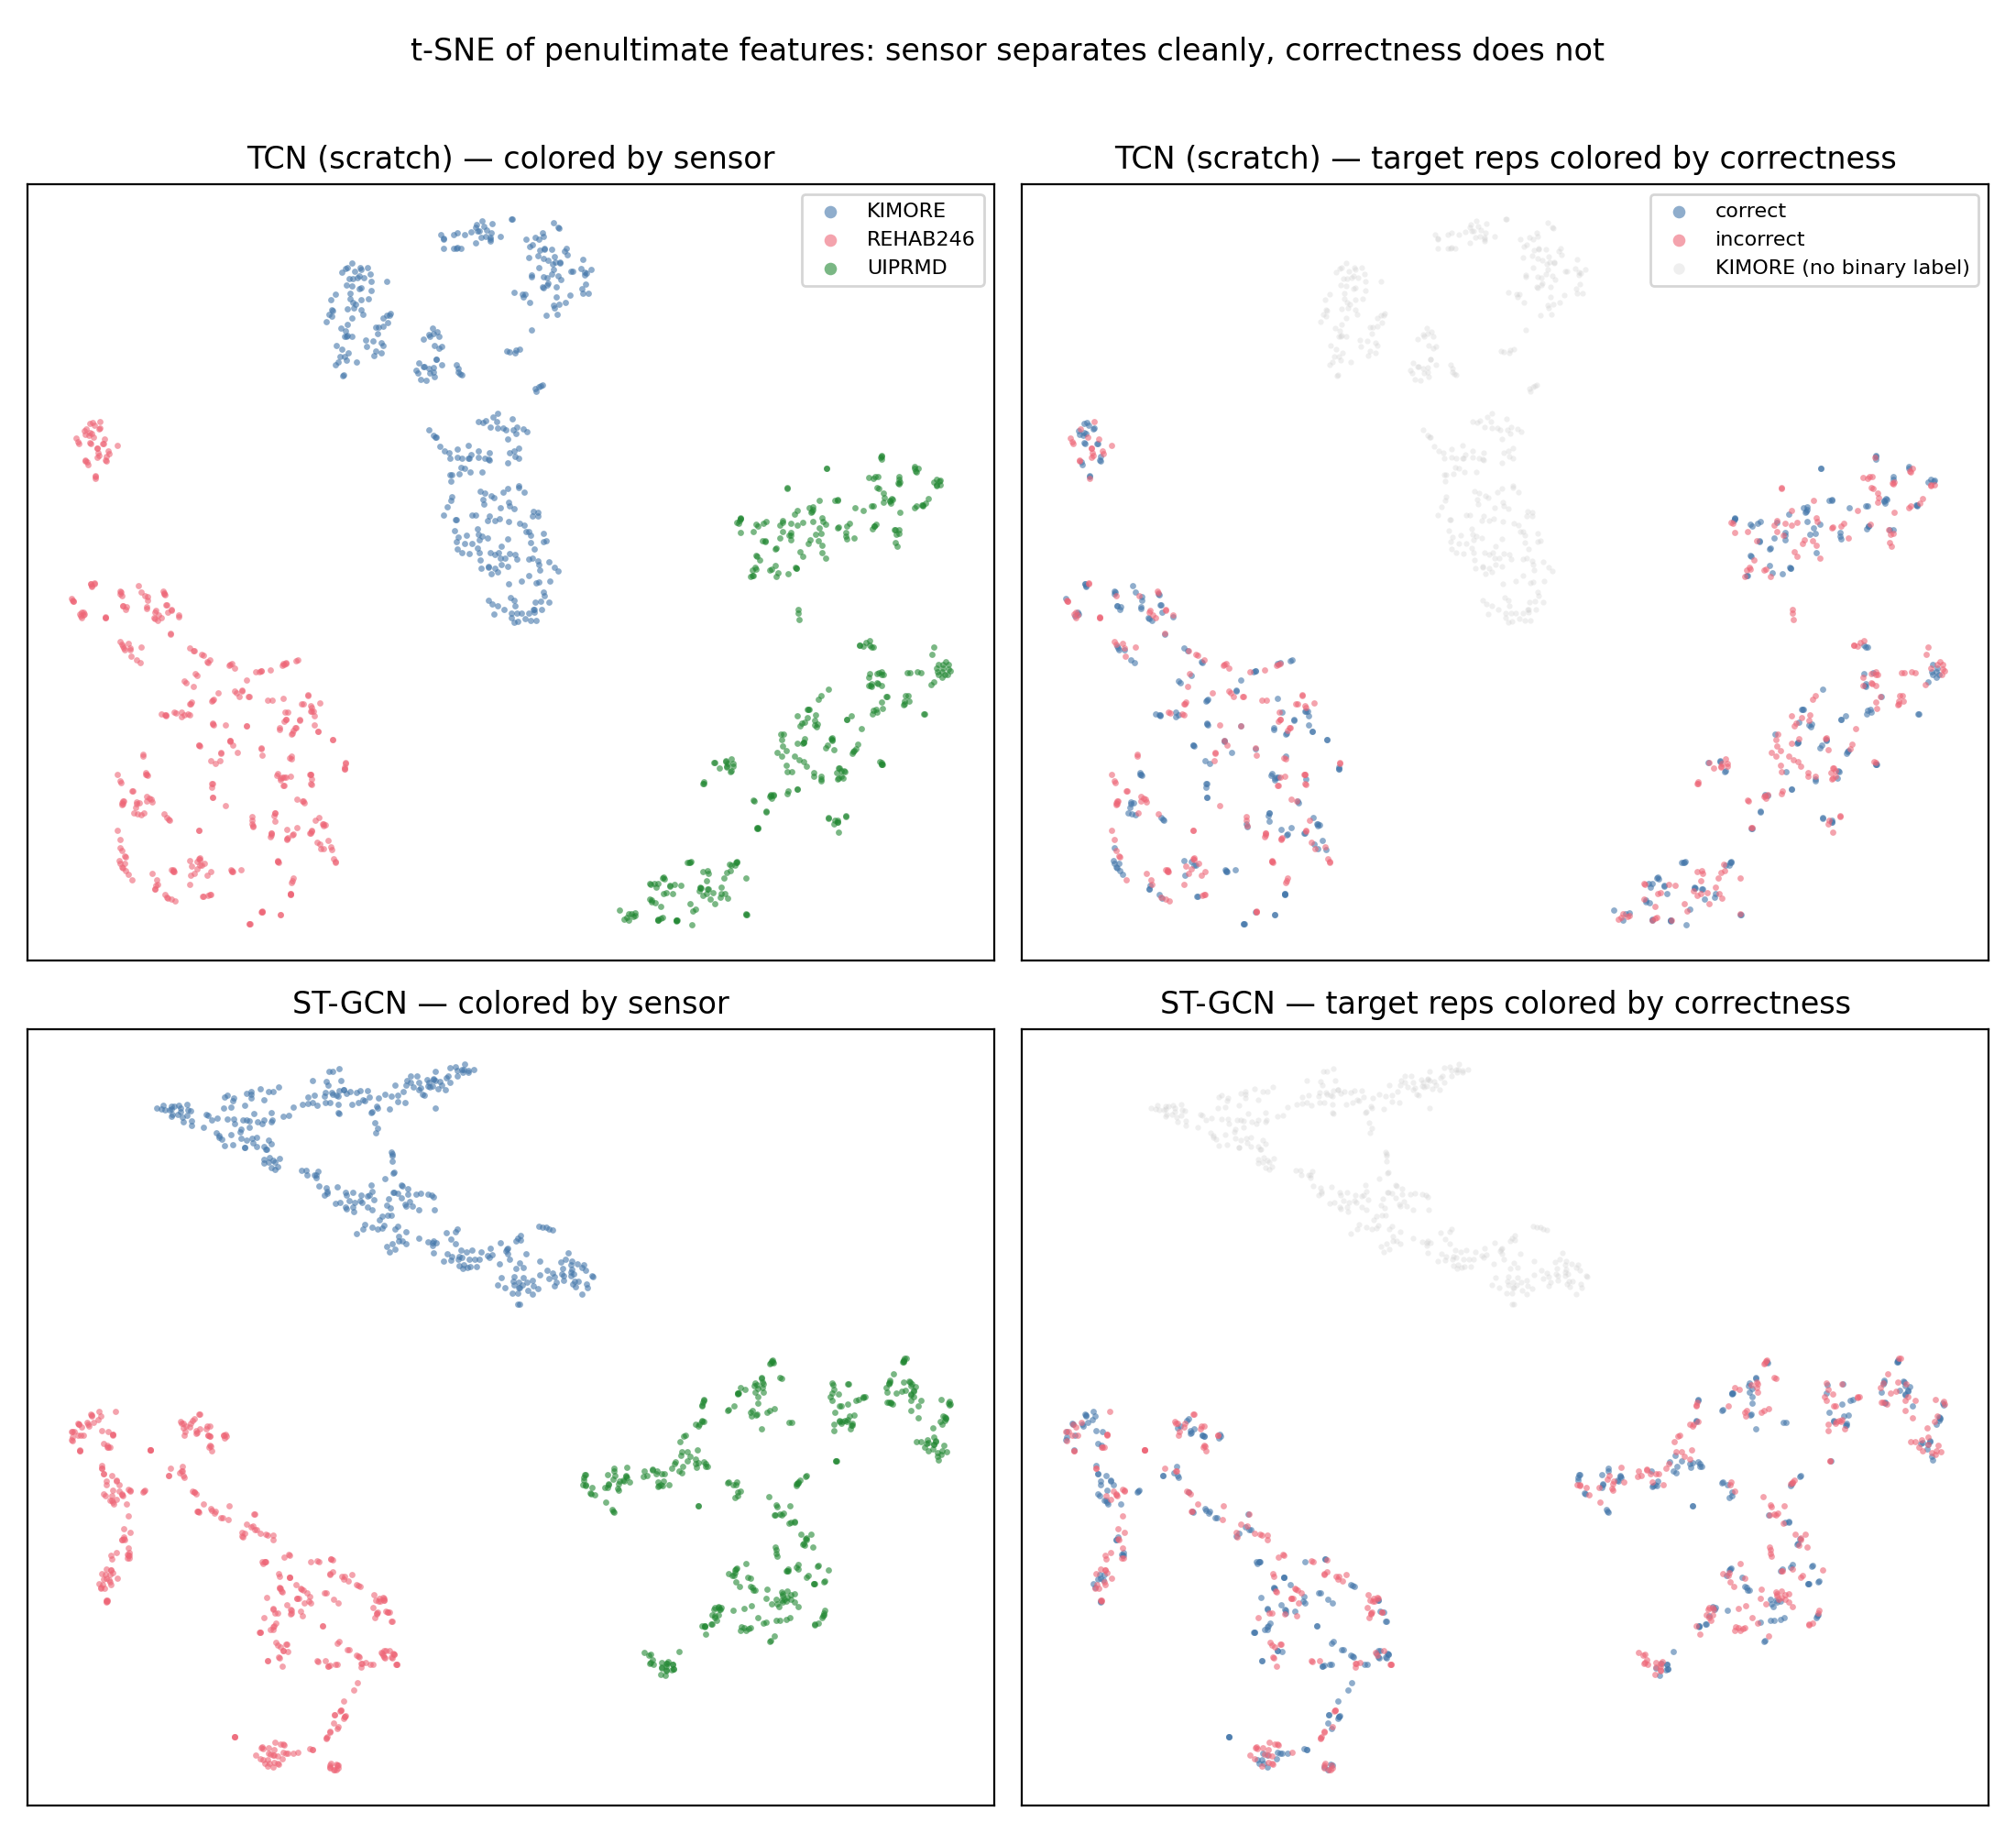
\includegraphics[width=\textwidth]{figures/embedding_tsne.png}
\caption{t-SNE of penultimate features on pooled KIMORE, REHAB246, and UI-PRMD sequences, for the scratch TCN (top) and ST-GCN (bottom). \textbf{Left:} colored by acquisition sensor --- the three corpora form cleanly separated clusters for both backbones, the visual counterpart of the perfect ($1.00$) sensor-identity probe. \textbf{Right:} the same embedding with target repetitions colored by correctness label (KIMORE, in grey, has no binary label); correct and incorrect repetitions are intermixed within each sensor cluster. The encoders organize features by sensor, not by movement quality.}
\label{fig:embedding-tsne}
\end{figure*}

\textbf{Few-shot calibration:} We probed whether 1, 5, 10, or 20 labeled target-sensor samples are needed to calibrate a logistic regression on frozen TCN features. For all the conditions and both corpora, few-shot AUROC is still at chance (0.51--0.54 even at $n = 20$), with $n = 1$ failing to yield a two-class evaluation. The 20-shot regime falls below the naive baseline (0.55/0.54), suggesting that even a modest handful of labelled target examples cannot compensate for the cross-sensor gap.

\textbf{Partial fine-tuning:} Freezing early TCN blocks (the input projection layer alone or blocks 0--1) during fine-tuning on the KIMORE data using all-corpora SSL encoders yields AUROCs of 0.50--0.56 --- still at chance. Overfitting to Kinect v2 statistics is not prevented by partial adaptation of the earliest layers.

\textbf{Naive-baseline sensitivity (joint padding and normalization).} Because the naive kinematic baseline is based on the harmonized 25-joint sequence, we have confirmed that it is not an artefact of joint padding or normalization (Table~\ref{tab:naive-sens}). Restriction of the features to truly distinct joints excluding three padded slots of UI-PRMD and four duplicated permutation targets (thumb${=}$wrist) of REHAB246 leaves the baseline essentially the same (REHAB246 $0.554 \to 0.548$; UI-PRMD identical at $0.538$, since a difference-based path/speed feature of all-zeros joint contributes exactly zero). Re-computation of learned models' consume drops REHAB246 to chance ($0.510$) while UI-PRMD is unchanged ($0.542$): the edge of the naive baseline on REHAB246 lies exactly in the global scale/speed cue whose loss we argued affects the cross-sensor transfer negatively (Section~\ref{sec:datasets}). Crucially, even on normalized coordinates the naive baseline is not below the learned models, so the learned conditions are not disadvantaged by the comparison.

\begin{table}[t]
\centering
\caption{Naive-baseline sensitivity to joint padding and normalization (zero-shot AUROC). ``Shared joints'' drops zero-padded (UI-PRMD) and duplicated (REHAB246) joints; ``z-scored'' recomputes features on per-sequence normalized coordinates.}
\label{tab:naive-sens}
\begin{tabular}{lccc}
\toprule
Corpus & Raw, all 25 & Shared joints only & Per-seq.\ z-scored \\
\midrule
REHAB246 & 0.554 & 0.548 & 0.510 \\
UI-PRMD  & 0.538 & 0.538 & 0.542 \\
\bottomrule
\end{tabular}
\end{table}

\subsection{Architecture, Representation, and Domain Adaptation}
\label{sec:robustness-c}
To test whether the null hypothesis is specific to the TCN backbone, the coordinate input, or the weak (CORAL) adaptation baseline, we repeated the zero-shot evaluation under several stronger settings (Table~\ref{tab:robustness-c}). (i) A spatial-prior \textbf{ST-GCN}~\cite{yan2018stgcn} backbone, trained under the identical 77-fold LOSO, remains at chance (REHAB246 $0.522\pm0.008$; UI-PRMD $0.514\pm0.010$) and below the naive baseline; crucially, 3-way sensor-identity probe on ST-GCN embeddings remains \emph{perfect} (balanced accuracy $1.00$ vs.\ chance $0.33$), confirming that sensor entanglement is not a TCN artifact but architecture independent. (ii) Bone-length-preserving \textbf{relative-joint-vector input} (each joint expressed relative to its skeletal parent; translation-invariant), used as the native model input rather than the post-hoc one, does not help (REHAB246 $0.534\pm0.017$; UI-PRMD $0.520\pm0.015$) --- nominally the highest learned AUROC, but still below the naive baseline, and not evidence of transfer: the direction-agnostic $\max(\text{AUROC}, 1-\text{AUROC})$ metric is biased upwards above 0.5 by construction, and the corresponding rank-Spearman correlations ($0.05$ and $0.02$) confirm no ordinal transfer. (iii) Three stronger domain-adaptation and domain-generalization baselines --- parameter-free \textbf{AdaBN}~\cite{li2018adabn} (target BatchNorm re-estimation on the ST-GCN), \textbf{DANN}~\cite{ganin2016dann} (gradient-reversal domain-adversarial training), and \textbf{SWAD}~\cite{cha2021swad} (flat-minima domain generalization via dense stochastic weight averaging over the training tail) remain at chance (AdaBN $0.519$/$0.514$; DANN $0.529$/$0.509$; SWAD $0.507$/$0.502$, both non-degenerate). SWAD is the flat-minima method suggested in the reviewer's DA/DG family survey, and it fails to reach the naive baseline. (iv) Finally, replacement of the global train-fit standardization with strict \textbf{per-sequence z-scoring} --- the normalization suspected as potentially discarding transfer-relevant scale does not change the result, leaving it at chance (REHAB246 $0.539\pm0.023$; UI-PRMD $0.534\pm0.027$), so that the null hypothesis does not depend on the normalization scheme. Across every architecture, input representation, normalization, and adaptation method tested, no combination reaches the naive baseline, and the sensor identity signal persists.

\begin{table}[t]
\centering
\small
\setlength{\tabcolsep}{3pt}
\caption{Robustness of the zero-shot null to backbone, input representation, and domain adaptation/generalization. AUROC (mean $\pm$ std across 77 folds where applicable). D = degenerate ($\text{pred\_SD}<0.10$). Naive kinematic baseline: 0.554 (REHAB246) / 0.538 (UI-PRMD).}
\label{tab:robustness-c}
\begin{tabular}{@{}lcc@{}}
\toprule
Setting & REHAB246 & UI-PRMD \\
\midrule
ST-GCN backbone         & $0.522{\pm}0.008$ & $0.514{\pm}0.010$ (D) \\
\quad + AdaBN           & $0.519{\pm}0.009$ & $0.514{\pm}0.010$ \\
Rel.-joint input        & $0.534{\pm}0.017$ & $0.520{\pm}0.015$ (D) \\
Per-seq.\ z-score       & $0.539{\pm}0.023$ & $0.534{\pm}0.027$ \\
DANN                    & $0.529$           & $0.509$ \\
SWAD (flat-minima DG)   & $0.507$           & $0.502$ \\
\midrule
Naive kinematic         & \textbf{0.554}    & \textbf{0.538} \\
\bottomrule
\end{tabular}
\end{table}

ST-GCN sensor-identity probe: 3-way balanced accuracy $1.00$ (chance $0.33$), confirming the diagnosis as architecture-independent.

\subsection{77-Fold LOSO: SSL FT = Scratch, SSL LP Worse}
\label{sec:loso-results}

Table~\ref{tab:loso} shows the within-domain KIMORE results under fully-powered LOSO.

\begin{table}[t]
\centering
\small
\setlength{\tabcolsep}{3pt}
\caption{KIMORE 77-fold true LOSO. Mean Spearman $\rho$ with 95\% bootstrap CI. Holm-Bonferroni adjusted $p$ versus scratch from paired Wilcoxon on absolute error ($N=380$). MAE and RMSE are on the original 0--50 score scale.}
\label{tab:loso}
\begin{tabular}{@{}lccccc@{}}
\toprule
Cond. & MAE & RMSE & $\rho$ & 95\% CI & $p$ (adj) \\
\midrule
Scratch     & 3.73 & 5.50 & \textbf{0.836} & [0.785, 0.867] & --- \\
Masked FT   & 4.02 & 5.69 & 0.823          & [0.773, 0.854] & 0.32 \\
Contrast.~FT & 4.01 & 6.03 & 0.816         & [0.762, 0.851] & 0.32 \\
Contrast.~LP & 5.95 & 8.28 & 0.689         & [0.617, 0.738] & $3.4{\times}10^{-14}$ \\
Masked~LP   & 6.16 & 8.27 & 0.679          & [0.612, 0.727] & $7.3{\times}10^{-18}$ \\
\bottomrule
\end{tabular}
\end{table}

SSL fine-tuning (both contrastive and masked) is statistically indistinguishable from scratch (adjusted $p > 0.3$). SSL linear-probing is significantly \emph{worse} than scratch (adjusted $p < 10^{-13}$). The two SSL paradigms are not significantly different: contrastive FT vs.\ masked FT $p = 0.80$, with $\Delta_{\text{abs-err}} = -0.01$. For compactness Table~\ref{tab:loso} lists adjusted $p$ versus scratch only; the full 10-pair matrix (Table~\ref{tab:pairwise-full}) exhibits the same structure --- \{scratch, contrastive-FT, masked-FT\} are mutually indistinguishable ($p_{\text{adj}} \geq 0.3$), the two linear-probe conditions are mutually indistinguishable ($p_{\text{adj}} = 0.46$), and every fine-tune-or-scratch versus linear-probe pair is significant ($p_{\text{adj}} < 10^{-10}$).

\begin{table}[t]
\centering
\footnotesize
\setlength{\tabcolsep}{4pt}
\caption{Full 10-pair Holm-Bonferroni-corrected Wilcoxon matrix on KIMORE 77-fold LOSO absolute error ($N=380$). ``Winner'' is the lower-error condition. Scr = scratch, Con = contrastive, Msk = masked, FT = fine-tune, LP = linear-probe. The three conditions \{Scr, Con-FT, Msk-FT\} are mutually indistinguishable, as are the two linear-probe conditions; every remaining pair is significant.}
\label{tab:pairwise-full}
\begin{tabular}{llcc}
\toprule
Comparison & Winner & $p_{\text{adj}}$ & Sig. \\
\midrule
Scr vs.\ Con-LP    & Scr    & $3.4\times10^{-14}$ & yes \\
Scr vs.\ Con-FT    & Scr    & $0.318$             & no  \\
Scr vs.\ Msk-LP    & Scr    & $7.3\times10^{-18}$ & yes \\
Scr vs.\ Msk-FT    & Scr    & $0.318$             & no  \\
Con-LP vs.\ Con-FT & Con-FT & $1.9\times10^{-11}$ & yes \\
Con-LP vs.\ Msk-LP & Con-LP & $0.455$             & no  \\
Con-LP vs.\ Msk-FT & Msk-FT & $4.3\times10^{-12}$ & yes \\
Con-FT vs.\ Msk-LP & Con-FT & $5.7\times10^{-16}$ & yes \\
Con-FT vs.\ Msk-FT & Con-FT & $0.805$             & no  \\
Msk-LP vs.\ Msk-FT & Msk-FT & $8.3\times10^{-17}$ & yes \\
\bottomrule
\end{tabular}
\end{table}

The probe sanity check is critical: linear-probe $\rho = 0.689$ (contrastive) and $0.679$ (masked) are considerably above zero, confirming that encoders learned relevant kinematic structure. Therefore, the null hypothesis is not due to under-trained encoders. Our scratch LOSO $\rho = 0.836$ is not directly comparable to the $\rho = 0.744$ of Karlov et al.\ \cite{karlov2024} on KIMORE: their figure employs different architecture and training recipe under 5-fold cross-validation (which allows subject-identity leakage), whereas ours is true 77-fold LOSO. Both indices the within-domain fit under different protocols and neither bears on the cross-sensor null hypothesis, which is evaluated on entirely different corpora.

\begin{table}[t]
\centering
\caption{Pool size ablation. Mean Spearman $\rho$ under 5-fold cross-subject split for two pretraining pool sizes.}
\label{tab:pool}
\begin{tabular}{lcc}
\toprule
Condition & IRDS-only ($\sim$1k) & All-corpora ($\sim$5k) \\
\midrule
Scratch         & \textbf{0.614} & \textbf{0.614} \\
Contrastive FT  & 0.581          & 0.534 \\
Masked FT       & 0.568          & 0.556 \\
Masked LP       & 0.350          & 0.515 \\
Contrastive LP  & 0.499          & 0.499 \\
\bottomrule
\end{tabular}
\end{table}

\subsection{Scale Ablation: More Data Does Not Help}
\label{sec:scale}

Table~\ref{tab:pool} compares the two pretraining pools. Scratch wins by machine precision with approximately 4$\times$ more unlabeled data. Contrastive FT performance deteriorates with more data (0.581 $\to$ 0.534). The scratch baseline reproduces to machine precision across two independent runs (identical folds by design), confirming a clean comparison. This pre-empts the critique that the negative result is a data-scale artifact.

\subsection{Zero-Shot Protocol Invariance}
\label{sec:protocol-invariance}

The 5-fold cross-subject zero-shot results (from the scale-ablation experiment) are essentially identical to the 77-fold true LOSO results in Table~\ref{tab:zeroshot}. For instance, scratch on REHAB246: 0.515 (5-fold) vs.\ 0.516 (77-fold); scratch on UI-PRMD: 0.517 vs.\ 0.524. This protocol invariance confirms that the negative zero-shot result is not an artefact of insufficient statistical power or evaluation protocol.

\subsection{Robustness Summary}
\label{sec:robustness}

The null hypothesis holds across every dimension we tested:
\begin{itemize}
    \item \textbf{Pretext task:} contrastive $\approx$ masked ($p = 0.80$).
    \item \textbf{Pool composition:} IRDS-only $\approx$ all-corpora (scratch still wins).
    \item \textbf{Pool size:} $\sim$1k vs.\ $\sim$5k sequences --- no qualitative change.
    \item \textbf{External corpus:} REHAB246 (OptiTrack) and UI-PRMD (Kinect) --- both at chance, both below naive baseline.
    \item \textbf{Evaluation protocol:} 5-fold cross-subject vs.\ 77-fold LOSO --- same null hypothesis.
\end{itemize}

\subsection{Degeneracy Threshold Sensitivity}
\label{sec:deg-sensitivity}

The degeneracy gate ($\text{pred\_SD} > 0.10$) is applied throughout to exclude collapsed models. Table~\ref{tab:deg-sensitivity} explores alternative thresholds. On REHAB246, no condition is degenerate at any threshold $\leq 0.15$, confirming that the chance-level AUROC is a true transfer failure. On UI-PRMD, the degeneracy classification is robust: all four flagged models are degenerate at $\text{pred\_SD}$ thresholds $0.05$ through $0.10$ (their $\text{pred\_SD}$ values are 0.015--0.033), and raising the threshold to 0.15 or 0.20 will include only borderline Scratch condition ($\text{pred\_SD}=0.12$). The $\text{pred\_SD}=0.10$ threshold is conservative: it correctly separates variance-collapsed models ($\text{pred\_SD} \leq 0.03$) from functioning models ($\text{pred\_SD} \geq 0.10$) on both corpora.

\begin{table}[t]
\centering
\caption{Degeneracy classification under alternative $\text{pred\_SD}$ thresholds. D = degenerate at that threshold.}
\label{tab:deg-sensitivity}
\small
\begin{tabular}{@{}lccccc@{}}
\toprule
Threshold & $<$0.05 & $<$0.08 & $<$0.10 & $<$0.15 & $<$0.20 \\
\midrule
\multicolumn{6}{c}{\textbf{REHAB246}} \\
A.\ Scratch         & . & . & . & . & . \\
B.\ Contrastive LP  & . & . & . & . & D \\
C.\ Contrastive FT  & . & . & . & . & . \\
D.\ Masked LP       & . & . & . & D & D \\
E.\ Masked FT       & . & . & . & . & . \\
\midrule
\multicolumn{6}{c}{\textbf{UI-PRMD}} \\
A.\ Scratch         & . & . & . & D & D \\
B.\ Contrastive LP  & D & D & D & D & D \\
C.\ Contrastive FT  & . & . & . & . & . \\
D.\ Masked LP       & D & D & D & D & D \\
E.\ Masked FT       & D & D & D & D & D \\
\bottomrule
\end{tabular}
\end{table}

% ===================================================================
\section{Discussion}
\label{sec:discussion}

\subsection{Why SSL Fails Cross-Sensor}
\label{sec:why-fails}

The probe-sanity result (linear-probe $\rho \approx 0.68$) demonstrates that the SSL encoders learn meaningful structure from the unlabeled target-sensor data. However, this structure does not transfer to the scoring task on a different sensor. The explanation is compound domain shift: coordinate joint distributions, bone-length ratios, frame rates, and noise profiles of the three sensors (Kinect v2, OptiTrack, and UI-PRMD acquisition setup) differ from one another. Furthermore, the exercise compositions vary across corpora --- KIMORE contains five trunk and hip exercises, while REHAB246 and UI-PRMD contain additionally some lower-limb exercises (Sect.~\ref{sec:datasets}). Thus, the domain shift is not merely sensor type, but the combination of sensor type, acquisition protocol, and exercise distribution. As these factors cannot be varied separately in public corpora, we cannot assign the failure to one factor; the conclusion is that SSL pretraining on unlabeled skeletons does not overcome this compound domain shift.

Our result is consistent with Karlov et al.\ \cite{karlov2024}, who show that SSL pretraining on IRDS improves KIMORE fine-tuning \emph{within the same sensor modality} (Kinect v2 $\to$ Kinect v2). The missing cell, which we fill, is cross-sensor zero-shot, where no improvement is observed. Together, the two results suggest that SSL effectively learns sensor-specific structure, but does not learn sensor-invariant representations of movement quality. Several further analyses support this interpretation.

First, the sensor-identity probe achieves perfect 3-way classification accuracy (1.00 vs.\ chance 0.33) on TCN features across KIMORE, REHAB246, and UI-PRMD and, identically (1.00), on ST-GCN features (Section~\ref{sec:robustness-c}) showing empirically that the encoder features encode sensor identity, not just movement quality, regardless of backbone. Second, CORAL \cite{sun2016deep} --- aligning second-order feature statistics from labeled KIMORE data before logistic regression on target features --- also fails (AUROC~0.52). Third, canonical input representations (pelvis-centering and bone-length normalization) applied without retraining do not improve any condition. Fourth, few-shot calibration with up to 20 labeled target samples stays at chance (AUROC~0.51--0.54), and partial fine-tuning that freezes early TCN blocks is equally ineffective (AUROC~0.50--0.56). The shift is deeper than coordinate-frame differences, implying that sensor-specific noise patterns, joint-angle distributions, and exercise composition are the key barriers.

\subsection{Why SSL Models Collapse on UI-PRMD}
\label{sec:collapse}

One conspicuous aspect of the results shown in Table~\ref{tab:zeroshot} is that four of five SSL conditions are degenerate ($\text{pred\_SD} < 0.10$) on UI-PRMD, while the scratch model only barely passes the threshold ($\text{pred\_SD}=0.12$, non-degenerate). This asymmetrical collapse --- SSL-pretrained models losing predictive variance on a same-sensor (Kinect v2) but different-acquisition corpus needs explanation.

Quantitatively, the collapsed SSL models on UI-PRMD produce predictions with $\text{pred\_SD} \approx 0.015$--$0.033$, compared with $\text{pred\_SD} \approx 0.10$--$0.67$ on REHAB246 for the same models. The output means also are shifted: the UI-PRMD predictions are clustered around 0.30--0.35 irrespective of the ground-truth label, while the predictions on REHAB246 span the whole score range. This is consistent with the hidden-state distribution shift: the SSL-encoder features, tuned to Kinect v2 statistics from IRDS and KIMORE, lie in a different part of the representation space on UI-PRMD although the sensor type nominally is the same, and the regressor head, trained on KIMORE representations, maps this shifted distribution into a narrow output range.

The IRDS pretraining corpus encodes Kinect v2-specific noise patterns, joint-angle distributions, and frame-rate characteristics. When the SSL encoder is then fine-tuned on KIMORE (also Kinect v2), it overfits to these sensor-specific features. On UI-PRMD, which is the same sensor type, but acquired in another room, in a different manner, with different calibration and subject population --- these overfitted features produce out-of-distribution hidden states, mapped to the narrow output range by the regressor head. The scratch model, initialized randomly, has no pretraining bias and thus preserves marginal predictive variance, although the AUROC of the model stays at chance level. This hypothesis is supported by the REHAB246 results: on a truly different sensor (OptiTrack), all the models are non-degenerate, as expected, with the pretraining having fitted no OptiTrack-specific artifacts.

\subsection{Implications for the Field}
\label{sec:implications}

This negative result is, we argue, more important than a positive one. It directs the research efforts from SSL architecture search (which pretext task, which augmentation, which pooling strategy) to the problem of sensor-invariant representation learning. The promising directions include:
\begin{itemize}
    \item Sensor-adversarial or invariance-based training which goes beyond the single-source DANN, CORAL, and SWAD baselines used in the paper (Section~\ref{sec:robustness-c}) --- for instance, adversarial training objectives across many sensors simultaneously.
    \item Multi-sensor pretraining which involves simultaneous pooling of Kinect, OptiTrack, and consumer web-camera skeletons during SSL, providing explicit cross-sensor variability to the encoder.
    \item Canonical body-model representations (e.g., SMPL \cite{loper2015smpl}) which remove sensor-specific pose estimation artifacts prior to the application of the scoring model.
\end{itemize}

\subsection{Rigor Contributions}
\label{sec:rigor}

Several design choices enhance the reliability of this negative result for TNSRE reviewers: (1) true 77-fold LOSO eliminates the subject-identity leakage; (2) the degeneracy criterion ($\text{pred\_SD} > 0.10$) prevents collapsed models from inflating the performance estimate; (3) naive kinematic baselines provide the simplest possible comparison anchor; (4) Holm-corrected sample-level tests ($N = 380$) avoid under-powered fold-level comparisons typical of the literature; and (5) the scale ablation and protocol-invariance analysis prevent the most likely critiques.

\subsection{Limitations}
\label{sec:limitations}

First, we evaluate only a single backbone architecture (TCN). Although the TCN is the best performing KIMORE architecture, spatial modeling backbones (ST-GCN \cite{yan2018stgcn}, Transformers with structural priors) may learn better sensor-invariant representations. Absence of the spatial priors may particularly hurt cross-sensor generalization because the different sensors generate different joint-coordinate artifacts which can be removed by the graph or attention mechanism. Second, we use only two SSL paradigms (contrastive and masked-motion); the skeleton-specific SSL methods like SkeletonCLR \cite{thoker2021skeletonclr} or cross-view contrastive learning could behave differently. Third, IRDS is the only unlabeled Kinect corpus of meaningful size; the results may not generalize to other Kinect-like sensors or to entirely different modalities (e.g., IMU, radar). Fourth, REHAB246 is marker-based (OptiTrack), not a consumer sensor; it represents the hardest zero-shot test. Fifth, UI-PRMD's ``incorrect'' class contains suboptimal execution by healthy subjects, not clinically graded errors; this may weaken the signal. Sixth, KIMORE's sample size ($n = 77$ subjects) limits statistical power of subgroup analyses; SSL may be helpful even at lower subject counts ($\sim$20 or below).

Seventh, our augmentation set does not include the temporal warping and bone-length preserving transforms; these skeleton-specific invariances \cite{thoker2021skeletonclr} --- designed to simulate variable speed and anthropometrics --- may improve cross-sensor transfer, but were not tested here. Eighth, the KIMORE continuous physician score (0--50) and binary correctness labels on target corpora are semantically mismatched; however, restricting evaluation to biomechanically overlapping exercises did not change the chance-level outcome, and AUPRC (which is robust to label mismatch and class imbalance) consistent with AUROC (0.51--0.54). We further tested the reviewer-suggested remedy directly: isotonic (monotone) calibration of KIMORE predictions and subsequent application to the target scores keeps both corpora at chance (REHAB246 $0.516 \to 0.517$; UI-PRMD $0.524 \to 0.504$ across 77 folds), proving that the source/target label-scale mismatch is not the reason of the null.

Ninth, besides the canonicalization ablations and CORAL, we tested several stronger remedies --- ST-GCN backbone, bone-length-preserving relative-joint-vector input, AdaBN, DANN, and SWAD (Section~\ref{sec:robustness-c}) --- and none was able to overcome the compound domain shift. Our adaptation baselines were chosen as one representative per methodological family: CORAL \cite{sun2016deep} for moment-matching (second-order feature-statistic alignment), AdaBN \cite{li2018adabn} for normalization statistics adaptation, DANN \cite{ganin2016dann} for adversarial feature alignment, and SWAD \cite{cha2021swad} for flat-minima domain generalization; together they cover the main families of unsupervised domain adaptation and generalization. Two further paradigms do not clearly apply to our single-source labeled regression setting: invariant-risk minimization (IRM) \cite{arjovsky2019irm} requires two or more labeled training domains, while we have a single labeled source (KIMORE); and test-time entropy minimization (TENT) \cite{wang2021tent} is defined for classification entropy, while our head is a scalar regressor --- AdaBN is the appropriate test-time adaptation for regression, but still stays at chance. Further, we note that the perfect sensor-identity probe (Section~\ref{sec:zeroshot-results}) localizes the failure in the learned representation, so the barrier seems representational and not a question of a particular alignment objective; multi-sensor pretraining (training the encoder on multiple sensors simultaneously) is thus the principal direction untested. Tenth, while we probe light-touch few-shot calibration (1--20 labeled target samples, Section~\ref{sec:zeroshot-results}) and find it staying at chance, we do not explore larger calibration budgets ($n > 20$) or active sample selection, which established domain adaptation literature suggests may eventually help the cross-sensor scoring. Establishing the data-efficiency boundary, below which the transfer becomes feasible, is the necessary next step before extending the negative result beyond the low-shot regime. Eleventh, our subject-level cross-sensor significance tests (Section~\ref{sec:zeroshot-results}, Table~\ref{tab:auroc-sig}) bootstrap over the ten subjects in each target corpus; ten clusters is a small sample size, so the corresponding confidence intervals are wide and the finding of the learned models being indistinguishable from chance is an absence of evidence limited by statistical power. LARGER multi-subject target corpora will make these intervals tighter, but the near-chance point estimates and the perfect sensor-identity probe make an alternative conclusion unlikely.

\subsection{Future Work}
\label{sec:future}

Besides the directions mentioned in Section~\ref{sec:implications}, we define four specific next steps: (1) a controlled comparison of SSL pretraining to supervised pretraining on a large labeled Kinect corpus to isolate the effect of label supervision; (2) demographic and clinical subgroup analysis to determine whether SSL differentially benefits specific patient populations; (3) multi-sensor pretraining and multi-domain generalization (e.g.,\ IRM \cite{arjovsky2019irm} with several labeled source sensors) --- the principal untested directions, since the single-source alignment (CORAL, AdaBN, DANN) and flat-minima generalization (SWAD) did not suffice (Section~\ref{sec:robustness-c}); and (4) largere budget and active few-shot calibration ($n > 20$ labeled target-sensor samples, extending the light-touch 1--20-shot probe of Section~\ref{sec:zeroshot-results}) to establish the data-efficiency boundary, below which the cross-sensor transfer becomes feasible.

% ===================================================================
\section{Conclusion}
\label{sec:conclusion}

We systematically tested whether the self-supervised pretraining on unlabeled skeletons from a different sensor allows zero-shot cross-sensor rehabilitation quality assessment. For two pretext tasks, two pool sizes (approximately 1,000 and 5,000 sequences), two independent labeled test corpora (REHAB246, OptiTrack; UI-PRMD, Kinect), and both 5-fold and 77-fold leave-one-subject-out protocols, the result is a clean negative: every SSL condition scores at chance cross-sensor (AUROC 0.51--0.53), and the within-domain (KIMORE) SSL fine-tuning is statistically indistinguishable from training from scratch while SSL linear-probing is significantly worse. Naive kinematic baseline leads nominally cross-sensor (0.55/0.54), but the bootstrap over the ten target subjects shows that neither the learned models nor the baseline achieve cross-sensor discrimination that is reliably above chance and mutually distinguishable. Quadrupling the unlabeled pool does not help. The barrier is the compound domain shift: encoders learn useful but sensor-specific structure (probe-sanity passes), and this structure does not transfer across sensors. This shift is multifaceted --- involving the sensor hardware, acquisition protocol, and exercise composition --- and SSL pretraining on unlabeled skeletons from a single sensor does not overcome it. We conclude that SSL pretraining on unlabeled skeletons is not a feasible approach for cross-sensor rehabilitation scoring, and recommend the field to prioritize the development of sensor-invariant representations --- whether by adversarial domain adaptation, multi-sensor pretraining, or canonical body models --- instead of more sophisticated SSL on a single sensor modality.

\subsection*{Code and Data Availability}
The KIMORE, IRDS, REHAB246, and UI-PRMD datasets are publicly available from their respective repositories. Pretraining, fine-tuning, and evaluation source code including fixed LOSO splits, joint mapping utilities, and preprocessing scripts will be made available at \url{https://github.com/opin-novice/Rehabilitation} upon acceptance of the paper.

% ===================================================================
\begin{thebibliography}{00}

\bibitem{capecci2019kimore}
M.~Capecci, M.~G.~Ceravolo, F.~Ferracuti, S.~Iarlori, A.~Monteriu, L.~Romeo, and F.~Verdini,
``The KIMORE dataset: Kinematic assessment of movement and clinical scores for remote monitoring of physical rehabilitation,''
\textit{IEEE Trans. Neural Syst. Rehabil. Eng.}, vol.~27, no.~7, pp.~1436--1448, 2019.

\bibitem{karlov2024}
M.~Karlov, A.~Abedi, and S.~S.~Khan,
``Rehabilitation exercise quality assessment through supervised contrastive learning with hard and soft negatives,''
\textit{Med. Biol. Eng. Comput.}, 2024.

\bibitem{abedi2023}
A.~Abedi, M.~Malmirian, and S.~S.~Khan,
``Cross-modal video to body-joints augmentation for rehabilitation exercise quality assessment,''
arXiv:2306.09546, 2023.

\bibitem{kuang2026}
Z.~Kuang, Y.~Yin, Y.~Yang, J.~Zhao, and L.~Sun,
``Dual-stream STGCN with motion-aware grouping for rehabilitation action quality assessment,''
\textit{Sensors}, vol.~26, no.~1, p.~287, 2026.

\bibitem{rehabpile2026}
A.~Ismail-Fawaz et al.,
``Rehab-Pile: A cross-subject rehabilitation benchmark aggregating KIMORE, UI-PRMD and IRDS,''
arXiv:2507.21018, IEEE FG 2026.

\bibitem{rehab246}
``REHAB246: An OptiTrack motion capture dataset for rehabilitation exercise assessment,''
Zenodo, 2025.

\bibitem{vakanski2018uiprmd}
A.~Vakanski, H.-P.~Jun, D.~Paul, and R.~Baker,
``A data set of human body movements for physical rehabilitation exercises (UI-PRMD),''
\textit{Data}, vol.~3, no.~1, p.~2, 2018.

\bibitem{bai2018tcn}
S.~Bai, J.~Z.~Kolter, and V.~Koltun,
``An empirical evaluation of generic convolutional and recurrent networks for sequence modeling,''
arXiv:1803.01271, 2018.

\bibitem{chen2020simclr}
T.~Chen, S.~Kornblith, M.~Norouzi, and G.~Hinton,
``A simple framework for contrastive learning of visual representations,''
in \textit{Proc. ICML}, 2020.

\bibitem{he2022mae}
K.~He, X.~Chen, S.~Xie, Y.~Li, P.~Doll\'{a}r, and R.~Girshick,
``Masked autoencoders are scalable vision learners,''
in \textit{Proc. CVPR}, 2022.

\bibitem{yan2018stgcn}
S.~Yan, Y.~Xiong, and D.~Lin,
``Spatial temporal graph convolutional networks for skeleton-based action recognition,''
in \textit{Proc. AAAI}, 2018.

\bibitem{ganin2016dann}
Y.~Ganin et al.,
``Domain-adversarial training of neural networks,''
\textit{J. Mach. Learn. Res.}, vol.~17, no.~1, pp.~2096--2130, 2016.

\bibitem{loper2015smpl}
M.~Loper, N.~Mahmood, J.~Romero, G.~Pons-Moll, and M.~J.~Black,
``SMPL: A skinned multi-person linear model,''
\textit{ACM Trans. Graph.}, vol.~34, no.~4, pp.~1--16, 2015.

\bibitem{sun2016deep}
B.~Sun, J.~Feng, and K.~Saenko,
``Deep CORAL: Correlation alignment for deep domain adaptation,''
in \textit{Proc. ECCV}, 2016.

\bibitem{long2015dan}
M.~Long, Y.~Cao, J.~Wang, and M.~I.~Jordan,
``Learning transferable features with deep adaptation networks,''
in \textit{Proc. ICML}, 2015.

\bibitem{li2018adabn}
Y.~Li, N.~Wang, J.~Shi, X.~Hou, and J.~Liu,
``Adaptive batch normalization for practical domain adaptation,''
\textit{Pattern Recognit.}, vol.~80, pp.~109--117, 2018.

\bibitem{liang2020shot}
J.~Liang, D.~Hu, and J.~Feng,
``Do we really need to access the source data? Source hypothesis transfer for unsupervised domain adaptation,''
in \textit{Proc. ICML}, 2020.

\bibitem{wang2021tent}
D.~Wang, E.~Shelhamer, S.~Liu, B.~Olshausen, and T.~Darrell,
``Tent: Fully test-time adaptation by entropy minimization,''
in \textit{Proc. ICLR}, 2021.

\bibitem{arjovsky2019irm}
M.~Arjovsky, L.~Bottou, I.~Gulrajani, and D.~Lopez-Paz,
``Invariant risk minimization,''
\textit{arXiv preprint arXiv:1907.02893}, 2019.

\bibitem{cha2021swad}
J.~Cha, S.~Chun, K.~Lee, H.-C.~Cho, S.~Park, Y.~Lee, and S.~Park,
``SWAD: Domain generalization by seeking flat minima,''
in \textit{Proc. NeurIPS}, 2021.

\bibitem{thoker2021skeletonclr}
F.~M.~Thoker \emph{et al.},
``SkeletonCLR: A contrastive representation learning framework for skeleton-based action recognition,''
in \textit{Proc. BMVC}, 2021.

\end{thebibliography}

\end{document}
